
\chapter{Introduzione}

\section{Reti Wireless}
Qualunque comunicazione avvenga tramite propagazione di onde nell'etere viene detta \textbf{Comunicazione Wireless}.

Essa è caratterizzata da:
\begin{itemize}
    \item \textbf{Frequenza Portante} e \textbf{Banda}
    \item \textbf{Potenza} del segnale
\end{itemize}

\subsection{Propagazione in spazio libero}
La potenza relativa ad un segnale radio in spazio libero segue questa formula:
\begin{equation*}
    P_r = P_t G_t G_r \left(\frac{\lambda}{4\pi d}\right)^2 = P_t G_t G_r \left(\frac{c}{4\pi d f_0}\right)^2
\end{equation*}

dove:
\begin{itemize}
    \item $f_0$ è la frequenza portante
    \item d è la distanza tra Tx e Rx
    \item $P_t$ e $P_r$ sono potenza trasmessa e potenza ricevuta
    \item $c = 3*10^8 m/s$
    \item $G_t$ e $G_r$ sono i guadagni in trasmissione e ricezione
\end{itemize}

Quindi la potenza si attenua con il \textbf{quadrato della distanza}.
\\
\subsection{Segmento di accesso}
Il territorio da coprire viene diviso in zone dette \textbf{celle} in cui vi è almeno una stazione \textbf{radio-base} (BS).
\begin{center}
    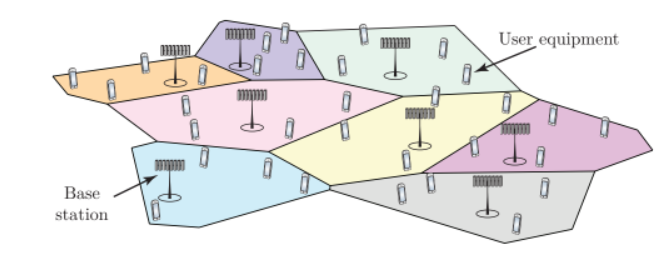
\includegraphics[width=\textwidth]{Images/Accass.png}
\end{center}

Differenziamo poi:
\begin{itemize}
    \item canale di \textbf{Uplink} (utenti mobili verso la stazione radio-base)
    \item canale di \textbf{Downlink} (stazione radio-base verso gli utenti mobili)
\end{itemize}

\section{Hand-off}
\textbf{L'Hand-off} è una procedura con cui un utente mobile viene sganciato da una BS e agganciato da un'altra.
\begin{center}
    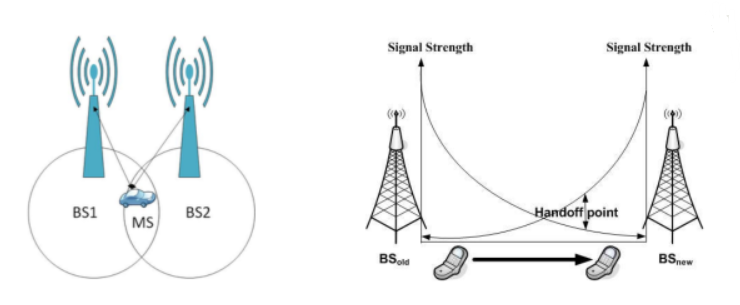
\includegraphics[width=\textwidth]{Images/HandOff.png}
\end{center}


Possiamo dividerlo in due categorie:
\begin{itemize}
    \item \textbf{Hard Hand-off}, in cui il terminale può essere servito SOLO da una BS
    \item \textbf{Soft Hand-off}, in cui il terminale può essere servito da due BS allo stesso tempo
\end{itemize}
%------------------------------------------------------------------------------------%

\section{Interferenza Multi Utente}
Dato che il canale Wireless è un mezzo di comunicazione \textbf{condiviso}, qualunque trasmissione sarà soggetta a \textbf{interferenze} dovute agli altri segnali degli \textbf{altri nodi della rete}. \\
Tipicamente ha una potenza \textbf{molto più significativa rispetto al rumore termico}, quindi è il problema principale da dover risolvere nelle trasmissioni Wireless, per questo motivo è necessario l'uso di tecniche di accesso multiplo.

\section{Tecniche di Accesso Multiplo}
\subsection{FDMA (Frequency Division Multiple Access)}
La \textbf{FDMA} (Frequency Division Multiple Access) assegna a ciascun utente una banda di frequenze dedicata:

\begin{center}
    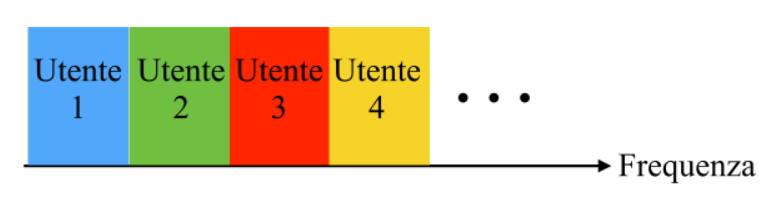
\includegraphics[width=\textwidth]{Images/FDMA.png}
\end{center}

Il ricevitore potrà così estrarre il segnale desiderato attraverso un \textbf{filtro passa-banda reale}.\\

\textit{\textbf{Tuttavia lo spettro di frequenze è limitato!!}} Quindi le bande di frequenza vengono riutilizzate tra celle non adiacenti, per far in modo che l'attenuazione del segnale dovuta alla distanza, non crei interferenza.
\\

\subsection{TDMA (Time Division Multiple Access)}
Il \textbf{TDMA} (Time Division Multiple Access) assegna a ciascun utente uno slot temporale dedicato:

\begin{center}
    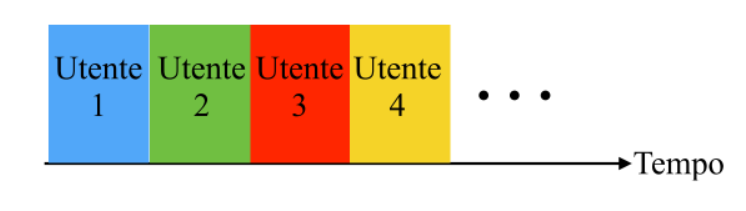
\includegraphics[width=\textwidth]{Images/TDMA.png}
\end{center}

Il ricevitore potrà così estrarre il segnale desiderato moltiplicando per un \textbf{impulso rettangolare}.
%------------------------------------------------------------------------------------%

\section{Fading}
Il segnale che parte dal trasmettitore si propagherà attraverso dei \textbf{cammini multipli} e ciò vuol dire che al ricevitore arriveranno delle \textbf{sovrapposizioni} del segnale trasmesso con \textbf{ritardi diversi}.\\

Questo effetto che caratterizza il Canale Wireless viene detto \textbf{Fading} e viene trattato come una realizzazione di una \textbf{variabile aleatoria}.
\\

\subsection{Path-Loss}
Il \textbf{Path-Loss} descrive l'assorbimento del segnale da parte degli oggetti presenti tra $T_x$ e $R_x$:
\begin{equation*}
    P_r = P_t G_t G_r \left(\frac{c}{4\pi f_0}\right)^2 \cdot \frac{1}{d^\eta}
\end{equation*}
\\

\subsection{Shadowing}
Lo \textbf{Shadowing} rappresenta anch'esso la densità di ostacoli tra $T_x$ e $R_x$, ma è modellata come una variabile aleatoria \textbf{log-normale}.
%------------------------------------------------------------------------------------%


\section{Canale Wireless}
Quindi sfruttando la sovrapposizione degli effetti possiamo rappresentare il segnale ricevuto nel seguente modo:
\begin{equation*}
    r(t) = \sum_{k=1}^K \alpha_k(t) \cdot s(t-\tau_k(t))
\end{equation*}
\\

\subsection{Doppler Spread}
Il \textbf{Doppler Spread} misura la selettività del canale dovuta alla tempo-varianza dei ritardi di propagazione:
\begin{equation*}
    D_s = \max_{i,j} \left|\tau_i^{'}(t) - \tau_j^{'}(t) \right| \cdot f_0
\end{equation*}
\\

\subsection{Tempo di Coerenza}
Il \textbf{Tempo di Coerenza} misura il tempo durante il quale il Canale Wireless si può ritenere stazionario:
\begin{equation*}
    T_c = \frac{1}{4D_s}
\end{equation*}
\\

\subsection{Multipath Delay Spread}
Il \textbf{Multipath Delay Spread} misura la selettività del canale dovuta alle differenze tra i ritardi di propagazione:
\begin{equation*}
    T_d = \max_{i,j} \left|\tau_i(t) - \tau_j(t) \right|
\end{equation*}
\\

\subsection{Banda di Coerenza}
La \textbf{Banda di Coerenza} misura la banda di frequenze in cui il Canale Wireless si può ritenere costante:
\begin{equation*}
    B_c = \frac{1}{2T_d}
\end{equation*}
\\

Una volta definite queste quantità, possiamo distinguere:
\subsection{Selettività}
\subsubsection{Selettività nel Tempo}
Sia $T_s$ il tempo di simbolo:
\begin{itemize}
    \item Se $T_c >> T_s$ si parla di \textbf{Flat Fading nel tempo}.
    \item Se $T_c << T_s$ si parla di \textbf{canale selettivo nel tempo}.
\end{itemize}

\subsubsection{Selettività in Frequenza}
Sia $B_s$ la banda:
\begin{itemize}
    \item Se $B_c >> B_s$ si parla di \textbf{Flat Fading in frequenza}.
    \item Se $B_c << B_s$ si parla di \textbf{canale selettivo in frequenza}.
\end{itemize}
%------------------------------------------------------------------------------------%
 


\section{Canale Flat Fading}
Consideriamo un canale \textbf{Flat Fading} nel \textbf{tempo} e in \textbf{frequenza}:
\begin{itemize}
    \item $T_c >> T_s$
    \item $B_c >> T_s$
\end{itemize}

L'effetto complessivo del Canale Wireless può essere espresso da un \textbf{singolo coefficiente aleatorio}:
\begin{equation*}
    h =\underbrace{\sqrt{G_t G_r} \left(\frac{c}{4\pi f_0}\right) \cdot \frac{1}{d^{\eta/2}}}_{Path-Loss} \underbrace{\psi}_{Shadowing} \underbrace{\delta}_{Fading}
\end{equation*}

\begin{itemize}
    \item $\psi$ è una v.a. log-normale
    \item $\delta \sim  CN(\mu,\sigma_\delta^2)$ 
\end{itemize}

\textit{\textbf{Quindi ogni $T_c$ si ha una nuova realizzazione di h!!}}
\\

\subsection{Fading di Rayleigh}
Nel caso in cui $\mu=0$, $|\delta|$ è distribuito come una variabile di \textbf{Rayleigh}.
\\

\subsection{Fading di Rice}
Nel caso in cui $\mu \neq 0$, $|\delta|$ è distribuito come una variabile di \textbf{Rice}.
%------------------------------------------------------------------------------------%


\section{Stima di Canale}
\begin{center}
    Come conoscere la realizzazione di h?
\end{center}

Essendo consci del fatto che h è costante durante il Tempo di Coerenza, trasmettiamo una sequenza di simboli noti (sequenza di training) $s_1,...,s_J$\\

Quindi riceveremo:
\begin{equation*}
    \vc{r} = \sqrt{p} h \vc{s} + \vc{n}= \begin{bmatrix}
    r_1\\.\\.\\.\\r_J
    \end{bmatrix}
 = \sqrt{p}h
     \begin{bmatrix}
    s_1\\.\\.\\.\\s_J
    \end{bmatrix} +
    \begin{bmatrix}
    n_1\\.\\.\\.\\n_J
    \end{bmatrix}
\end{equation*}

Moltiplicheremo poi il vettore $\vc{r}$ con il vettore $\vc{s}^H$:
\begin{equation*}
\begin{aligned}
    y &= \vc{s}^H \vc{r} = \sqrt{p} h ||\vc{s}||^2 + \vc{s}^H\vc{n} = \\[10pt]
    &=\sqrt{p}h||\vc{s}||^2 + w
\end{aligned}
\end{equation*}
\\
dove $w \sim  CN(0,\sigma^2 ||\vc{s}||^2) $

Quindi data la \textbf{sequenza di training} $\vc{s}$, usando metodi di stima possiamo ottenere una \textbf{stima di h}.\\

Tuttavia in ogni \textbf{intervallo di coerenza}, prima di poter iniziare a comunicare \textbf{bisogna stimarsi il canale h}.





